\documentclass[portuguese]{sbc2025}%

%\usepackage{graphicx}% já está incluido na classe
%\usepackage[utf8]{inputenc} % obsoleto, desnecessário

\usepackage[misc,geometry]{ifsym} 
\usepackage{hyperref}

%%%%  %\usepackage{fontspec}

%% Os problemas com a classe eram originados por carregarem ambos os
%% pacotes fontenc e fontspec simultaneamente. Agora a classe detecta
%% qual engine está em uso e se for o pdflates então carrega o
%% fontenc. Se forem o xelatex ou lualatex então carrega o
%% fontspec. Eu particularemnte prefiro o lualatex ou o xetex


% \usepackage{fontawesome} %%% incluido na classe. Desnecessário
% chamá-lo aqui


%%%% \usepackage{academicons}
%%%% outro encrenqueiro que se tornou desnecessario. Deste typeface só
%%%% se usava o glifo do orcid e o codigo interno bombava.
%%%% Substitui pelo pacote orcidlink (carregado internamete na classe)
%%%% e consertei o codigo na classe.


%\usepackage{color} % carregada dentro da classe
%\usepackage{hyperref} % carregada dentro da classe

\usepackage{aas_macros}
\usepackage[bottom]{footmisc}
\usepackage{float}
\usepackage{booktabs}

%\usepackage{supertabular}
%\usepackage{multicol}
%\usepackage{multirow}
%% O pacote tabularray é muito melhor para
% a criacao de tabela complexas e/ou loooongas; tudo de modo simples.
%% Torna o uso de multicol e multirow desnecessarios

\usepackage{tabularray}


\usepackage{afterpage}
\usepackage{url}
\usepackage{pifont}


\setcitestyle{square}


\definecolor{engtitle}{rgb}{0.5,0.5,0.5}
\definecolor{orcidlogo}{rgb}{0.37,0.48,0.13}
\definecolor{unilogo}{rgb}{0.16, 0.26, 0.58}
\definecolor{maillogo}{rgb}{0.58, 0.16, 0.26}
\definecolor{darkblue}{rgb}{0.0,0.0,0.0}
\hypersetup{colorlinks,breaklinks,
            linkcolor=darkblue,urlcolor=darkblue,
            anchorcolor=darkblue,citecolor=darkblue}
%\hypersetup{colorlinks,citecolor=blue,linkcolor=blue,urlcolor=blue}

%%%%%%% IMPORTANT: We disable hyperlinks by default with this line, to avoid the error "\pdfendlink ended up in different nesting level" while writing.
%\hypersetup{draft}

\category{Artigo de Pesquisa/Research Paper}
\title[Template SOL Preprints para trabalhos em português]{Análise do impacto de intervenções viárias no desempenho de uma rede urbana: um estudo de caso no Gama, DF}
%\engtitle{\textcolor{engtitle}{Aprimorando o planejamento viário com grafos e dados reais}}

%THE ORCID IS MANDATORY FOR EACH AUTHOR IN JBCS
\author[Marcinoni et al. 2026]{

\affil{\textbf{Pedro Marcinoni Varão Ribeiro Vieira da Rosa}
\\Universidade de Brasília~\ror{02xfp8v59}
\\\href{mailto:pedroextrer@gmail.com}{\textit{pedroextrer@gmail.com}}}

\affil{\textbf{Davi Brasileiro Gomes}
\\Universidade de Brasília~\ror{02xfp8v59}
\\\href{mailto:davi.brasileiro.gomes@gmail.com}{\textit{davi.brasileiro.gomes@gmail.com}}}

\affil{\textbf{Davi Galvão Guerra}
\\Universidade de Brasília~\ror{02xfp8v59}
\\\href{mailto:daviguerra27@gmail.com}{\textit{daviguerra27@gmail.com}}}

\affil{\textbf{Leonardo Mileo Moreira Krauss Guimarães}
\\Universidade de Brasília~\ror{02xfp8v59}
\\\href{mailto:leonardokrauss3107@gmail.com}{\textit{leonardokrauss3107@gmail.com}}}

\affil{\textbf{Patrícia Araújo de Oliveira}
\\Universidade de Brasília~\ror{02xfp8v59}
\\\href{patricia.oliveira@unb.br}{\textit{patricia.oliveira@unb.br}}}

}


\begin{document}

\begin{frontmatter}

\maketitle

\begin{abstract-pt}
Este artigo investiga o impacto de intervenções viárias no congestionamento e tempos de deslocamento, utilizando grafos direcionados para identificar gargalos urbanos. Modelou-se a região do trevo EPCT/EPIP/DF-480 com dados do OpenStreetMap e TomTom. O tráfego foi simulado com o algoritmo de Frank-Wolfe, considerando o equilíbrio de Wardrop e funções BPR. Foram avaliados cenários de adição, remoção e inversão de vias, comparando seus efeitos sobre o Tempo Total de Viagem do Sistema e o Índice de desempenho de velocidade. Os resultados indicam que a adição de capacidade reduziu o Tempo Total de Viagem (TSTT) em aproximadamente 8,5\%, enquanto intervenções restritivas, como a remoção e inversão de alças, pioraram o desempenho global, aumentando o TSTT em até 2,57\% e 3,23\%, respectivamente, ao sobrecarregar gargalos e vias locais. Conclui-se que vias com baixos índices de velocidade frequentemente cumprem a função vital de evitar a sobrecarga de corredores principais, e que a modelagem topológica por grafos é essencial para antecipar deteriorações sistêmicas que métricas isoladas de velocidade podem mascarar.
\end{abstract-pt}

\begin{keywords}
Índice de desempenho de velocidade, Tempo Total de Viagem do Sistema, Equilíbrio de Wardrop, Função Volume-Atraso, Algoritmo de Frank-Wolfe, Paradoxo de Braess
\end{keywords}


%\begin{license}
%Published under the Creative Commons Attribution 4.0 International Public License (CC BY 4.0)
%\end{license}

\end{frontmatter}


\section{Introdução}
\label{sec:intro}
O crescimento da demanda por mobilidade urbana exige um planejamento viário capaz de reduzir congestionamentos e melhorar os tempos de deslocamento. Nesse contexto, a identificação de gargalos e a avaliação dos efeitos de intervenções na malha viária são fundamentais para compreender o desempenho do sistema. Este estudo concentra-se na região do Gama, no Distrito Federal, especialmente no entroncamento entre a EPCT, a EPIP e a DF-480.

A pesquisa busca responder a duas questões: Como intervenções pontuais na malha viária afetam os tempos de deslocamento e o congestionamento nas vias adjacentes? Como a modelagem da infraestrutura viária por meio de grafos direcionados ponderados contribui para identificar gargalos e compreender as causas dos congestionamentos?

Para respondê-las, são integrados dados geográficos e de tráfego em um modelo de rede viária, permitindo simular intervenções de adição de faixas, remoção de ligações e inversão de sentido. Seus efeitos são avaliados por meio de indicadores de fluidez e tempo total de viagem, considerando tanto os trechos modificados quanto o desempenho global da rede e possíveis diferenças entre esses indicadores. O artigo, portanto, é dividido nos seguintes tópicos: 2. Fundamentação Teórica, 3. Metodologia, 4. Resultados, 5. Discussão e Limitação e 6. Conclusão e Trabalhos Futuros.
 
\section{Fundamentação Teórica}
Aqui são explorados os conceitos técnicos associados à análise de congestionamento viário necessários, tais como o Paradoxo de Braess, Equilíbrio de Wardrop, Função Volume-Atraso e Índice de Desempenho de Velocidade.

\subsection{Índice de Desempenho de Velocidade}
O Speed Performance Indicator (SPI) analisa o desempenho viário pela razão entre a velocidade média observada em uma via e sua velocidade máxima permitida \cite{he2016spi}. Aqui, o chamamos de K por facilidade.

\subsection{Equilíbrio do usuário de Wardrop}
O equilíbrio de Wardrop define a situação onde nenhum motorista pode, sozinho, reduzir seu tempo médio de deslocamento na malha apenas alterando o trajeto escolhido \cite{wardrop1952}.

\subsection{Função volume-atraso}
A Função Volume-Atraso (VDF), também chamada de função BPR, representa a variação do tempo de deslocamento considerando a razão entre volume de veículos e capacidade viária. É modelada como $t(v) = t_0 \cdot (1 + a(v/c)^b)$, sendo $a$ e $b$ coeficientes de calibração específicos de cada malha.

\subsection{Paradoxo de Braess}
Define a situação na qual adicionar uma nova via à malha pode não reduzir o congestionamento \cite{braess2005}, mas sim aumentá-lo, criando novos gargalos.

\section{Metodologia}
\label{sec:metodologia}

Esta seção apresenta uma descrição sobre a modelagem em grafo da área de estudos selecionada, a obtenção dos dados relacionados ao sistema viário da região, a implementação do algoritmo de alocação de tráfego e a formulação das propostas de intervenções no grafo.

\subsection{Visão geral e área de estudo}

Adotou-se um modelo de alocação estática de tráfego, representando a malha viária por um grafo direcionado com demanda fixa. As intervenções foram realizadas por alterações discretas no grafo \cite{leblanc1975dndp}, enquanto a redistribuição dos fluxos foi simulada pelo algoritmo de Frank-Wolfe \cite{leblanc1975fw}, considerando o equilíbrio de Wardrop \cite{wardrop1952} e a função volume-atraso BPR \cite{bpr1964}.

A área de estudo compreende o entorno do trevo entre a EPCT (DF-001), a EPIP e a DF-480, no Gama (DF). A rede foi obtida do OpenStreetMap por meio do OSMnx 2.1.1. O subgrafo inicial de 30 nós foi ampliado para incorporar rotas alternativas, utilizando vias de classe terciária ou superior contidas na envoltória convexa dos nós, com margem de 200~m. O grafo final possui 134 nós e 236 arestas, com 40,2\% da demanda dispondo de ao menos duas rotas competitivas.

\subsection{Demanda}

A demanda foi obtida pela ferramenta TomTom O/D Analysis, com regiões de origem e destino associadas aos 134 nós da rede e registros de 22 dias úteis de julho de 2026, entre 18h e 19h. As viagens externas foram associadas à primeira ou à última região atravessada. A partir dos percentuais fornecidos pela plataforma, foram reconstruídas 15.429 viagens, das quais 86\% correspondiam a tráfego de passagem. Após a exclusão de viagens intranó e pares sem caminho, restaram 14.960 viagens em 1.031 pares origem-destino.

Como a amostra representa apenas parte do tráfego real, aplicou-se um fator de expansão calibrado com a mediana das contagens volumétricas do DER-DF para o mesmo período. Calculado pela razão entre contagens do DER-DF em quatro pontos e fluxos da amostra, o fator variou de 8,82 a 21,96. Adotou-se a mediana (12,21; ou 8.309 veículos/h) no cenário-base, e os extremos para simular demandas baixa e alta.

\subsection{Atributos das arestas}

As velocidades foram obtidas do TomTom Traffic Stats para os dias úteis de julho de 2026, nos períodos de pico (18h--19h) e madrugada (0h--4h). Os registros foram associados às arestas conforme sua posição e sentido, calculando-se a velocidade pela média harmônica ponderada pelo comprimento sobreposto. O índice $K$ foi definido pela razão entre a velocidade de pico e o limite regulamentado da via \cite{he2016spi}.

Os limites de velocidade e o número de faixas foram extraídos do OSM e, quando ausentes, estimados com base nas características das vias e no Código de Trânsito Brasileiro \cite{ctb2026}. A capacidade de cada aresta foi calculada pelo número de faixas multiplicado pela capacidade por faixa, entre 600 e 1.800 veículos/h, conforme a classe viária. O tempo em fluxo livre foi estimado pela maior velocidade entre os períodos de pico e madrugada, limitada ao valor regulamentado.

Como a função BPR \cite{bpr1964}, com parâmetros clássicos ($a=0{,}15$ e $b=4$), subestimou os atrasos observados no trevo, foram ajustadas as capacidades efetivas de 25 arestas em que o fluxo estimado superava 30\% da capacidade nominal e o atraso observado excedia o previsto. O ajuste buscou reproduzir os tempos observados, respeitando o limite da capacidade nominal, embora parte da avaliação de consistência permaneça dependente da calibração.

\subsection{Alocação, cenários e indicadores}

O equilíbrio de Wardrop foi obtido pela formulação de Beckmann \cite{beckmann1956}, sujeita às restrições de conservação de fluxo. O algoritmo de Frank-Wolfe \cite{frank1956} parte da alocação em fluxo livre e atualiza iterativamente os tempos e caminhos mínimos, redistribuindo os fluxos até que o \textit{gap} relativo seja inferior a $10^{-4}$ ou o limite de 500 iterações seja atingido. O desempenho foi avaliado pelo índice $K_e=v_e/v_{\text{lim},e}$, com $v_e=L_e/t_e$, e pelo Tempo Total de Viagem do Sistema ($TSTT=\sum_e x_e t_e(x_e)$).

Foram simuladas intervenções de adição de faixas, remoção de arestas e inversão de sentido em trechos selecionados a partir dos indicadores de fluidez e fluxo. Seus efeitos foram comparados ao cenário-base, investigando-se possíveis deteriorações sistêmicas associadas ao Paradoxo de Braess \cite{braess2005}. As simulações consideraram três níveis de demanda e uma análise de sensibilidade aos parâmetros BPR ($a=0{,}8$ e $b=4{,}7$) \cite{vdf2023}, com as capacidades efetivas recalculadas.

\subsection{Limitações do desenho}

O modelo estático não considera a propagação de filas, os atrasos em semáforos ou rotas por vias locais, excluídas do grafo. Além disso, a predominância de viagens de passagem
limita as alternativas de rota disponíveis. As capacidades viárias foram estimadas com base na literatura, enquanto parte dos limites de velocidade e do número de faixas foi preenchida por estimativas. Por fim, a avaliação de consistência não constitui uma validação independente, pois os dados observados também foram utilizados na construção e calibração do modelo.

\section{Resultados}

\subsection{Diagnóstico inicial do K}
\label{sec:diagnostico_k}

A Fig.~\ref{fig:k_inicial} apresenta a distribuição espacial do índice $K$ no cenário-base, considerando o horário de pico (18h--19h).

\begin{figure}[H]
\centering
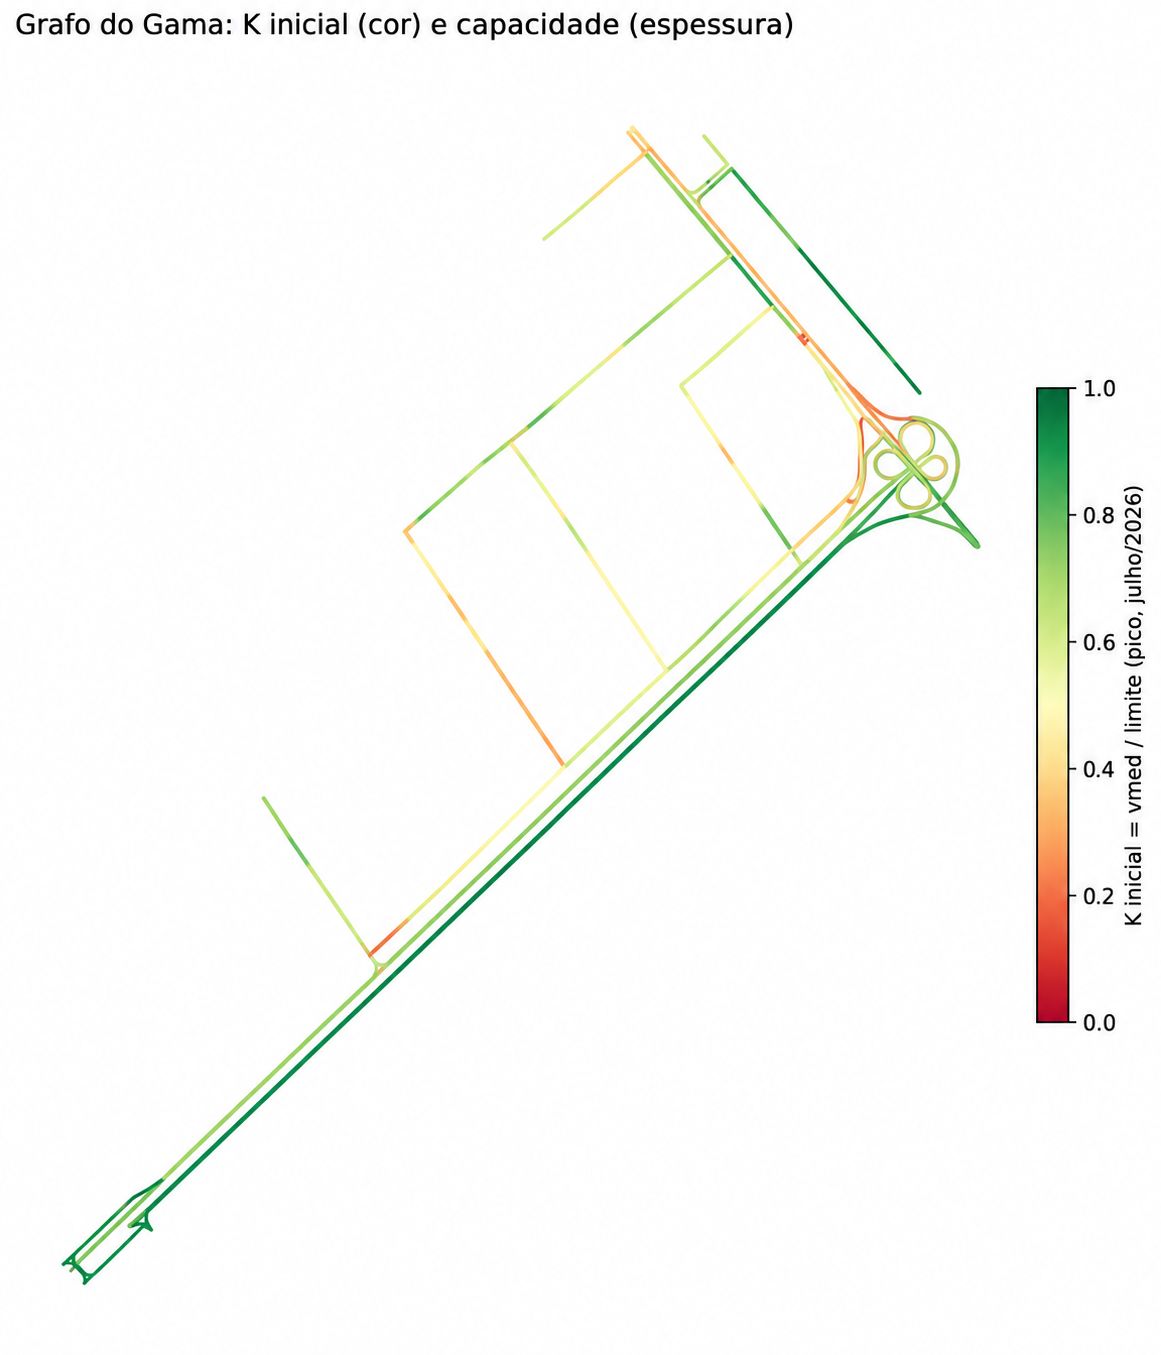
\includegraphics[width=4.3cm]{gama_drive_expanded_k_inicial_branco.png}
\caption{Distribuição espacial do índice $K$ na região do Gama (EPCT/EPIP/DF-480).}
\label{fig:k_inicial}
\end{figure}

A análise revela diferentes condições de circulação: as rodovias principais apresentam valores de $K$ superiores a $0{,}8$, indicando velocidades próximas aos limites regulamentados; as vias coletoras e conexões secundárias apresentam valores entre $0{,}4$ e $0{,}7$, indicando redução moderada das velocidades; e os gargalos mais críticos, que apresentam valores de $K$ inferiores $0{,}3$, a concentram-se no trevo entre a EPCT, a EPIP e a DF-480, especialmente nas alças de acesso.

\subsection{Convergência do Algoritmo}
O algoritmo de Frank-Wolfe foi empregado para obter uma solução aproximada do Equilíbrio de Wardrop na rede viária modelada. A Tabela~\ref{tab:convergencia_base} sintetiza a convergência computacional obtida nos três níveis de demanda no cenário-base.

\begin{table}[htbp]
\caption{Desempenho de Convergência do Algoritmo de Frank-Wolfe}
\label{tab:convergencia_base}
\centering
\resizebox{\columnwidth}{!}{%
\begin{tabular}{lcccc}
\hline
\textbf{Nível de Demanda} & \textbf{Fator} & \textbf{Iterações} & \textbf{\textit{Gap} Final} & \textbf{Tempo (s)} \\
\hline
Baixa & 8,82 & 2 & $3,5 \times 10^{-16}$ & 0,21 \\
Adotada & 12,21 & 4 & $3,1 \times 10^{-9}$ & 0,34 \\
Alta & 21,96 & 28 & $1,0 \times 10^{-4}$ & 2,23 \\
\hline
\end{tabular}%
}
\end{table}

A conferência com os dados reais de tráfego (nível de demanda adotada) demonstrou forte aderência: o fluxo modelado e as passagens TomTom em 40 arestas isoladas atingiu uma correlação de $0,93$, com $GEH$ mediano de $3,48$, e nas 130 arestas não calibradas, a razão mediana entre tempo modelado e observado foi de $0,912$.

\subsection{Análise dos Cenários}
A Tabela~\ref{tab:indicadores_base} apresenta os principais indicadores da malha viária atual nos três níveis de demanda.

\begin{table}[htbp]
\caption{Indicadores Macro do Sistema}
\label{tab:indicadores_base}
\centering
\resizebox{\columnwidth}{!}{%
\begin{tabular}{lccc}
\hline
\textbf{Indicador} & \textbf{D. Baixa} & \textbf{D. Adotada} & \textbf{D. Alta} \\
\hline
Demanda Total (veículos/h) & 6.002,2 & 8.309,2 & 14.944,3 \\
TSTT (veículos$\cdot$h) & 343,36 & 476,94 & 884,36 \\
Velocidade Média (km/h) & 45,20 & 45,05 & 43,68 \\
Tempo Médio de Viagem (min) & 3,43 & 3,44 & 3,55 \\
Índice de Fluidez Média ($K_{rede}$) & 0,7026 & 0,7001 & 0,6763 \\
Arestas Saturadas ($V/C > 1{,}0$) & 20 & 20 & 26 \\
Arestas Lentas ($K < 0{,}5$) & 67 & 67 & 68 \\
\hline
\end{tabular}%
}
\end{table}

Para avaliar as intervenções, selecionaram-se três cenários topologicamente distintos principais: 
\begin{itemize}
    \item \textbf{C0}: adiciona uma faixa, de duas para três, em cinco arestas-gargalo da EPCT Norte;
    \item \textbf{R3}: remove a alça de retorno $11\rightarrow63$ (que tinha o menor $K$ observado, $0{,}16$); e
    \item \textbf{S3}: inverte o sentido da alça de acesso à DF-480.
\end{itemize}
A conectividade dos 1.031 pares O-D foi mantida e os resultados estão consolidados na Tabela~\ref{tab:intervencoes}.

\begin{table}[htbp]
\caption{Impacto das três intervenções em relação à situação atual}
\label{tab:intervencoes}
\centering
\resizebox{\columnwidth}{!}{%
\begin{tabular}{llcccc}
\hline
\textbf{Intervenção} & \textbf{Demanda} & \textbf{TSTT (veículos$\cdot$h)} & \textbf{$\Delta$TSTT (\%)} & \textbf{$K_{rede}$ ($\Delta K$)} & \textbf{Arestas $V/C>1$} \\
\hline
C0: +1 faixa na EPCT Norte & Baixa & 313,85 & $-8{,}59$ & 0,7263 ($+0{,}0237$) & $20\rightarrow19$ \\
 & Adotada & 436,07 & $-8{,}57$ & 0,7238 ($+0{,}0237$) & $20\rightarrow19$ \\
 & Alta & 810,77 & $-8{,}32$ & 0,6999 ($+0{,}0236$) & $26\rightarrow25$ \\
\hline
R3: remoção da alça $11\rightarrow63$ & Baixa & 351,76 & $+2{,}45$ & 0,6990 ($-0{,}0036$) & $20\rightarrow20$ \\
 & Adotada & 488,71 & $+2{,}47$ & 0,6963 ($-0{,}0038$) & $20\rightarrow20$ \\
 & Alta & 907,12 & $+2{,}57$ & 0,6716 ($-0{,}0047$) & $26\rightarrow27$ \\
\hline
S3: inversão da alça de acesso à DF-480 & Baixa & 347,31 & $+1{,}15$ & 0,7047 ($+0{,}0021$) & $20\rightarrow17$ \\
 & Adotada & 484,30 & $+1{,}54$ & 0,7011 ($+0{,}0010$) & $20\rightarrow18$ \\
 & Alta & 912,91 & $+3{,}23$ & 0,6730 ($-0{,}0033$) & $26\rightarrow26$ \\
\hline
\end{tabular}%
}
\end{table}

A adição de capacidade (C0) reduziu o TSTT em cerca de 8,5\% nos três níveis e elevou o $K_{rede}$. Contudo, não eliminou a saturação (as arestas com $V/C>1$ caíram apenas de 20 para 19); o ganho veio da redução acentuada no tempo de atraso dado pela BPR. Já a remoção (R3) piorou tanto o TSTT ($+2{,}5\%$) quanto o $K_{rede}$. Por fim, a inversão (S3) apresentou divergência de indicadores nas demandas baixa e adotada: aumentou o TSTT (piora de 1,15\% e 1,54\%), mas elevou o $K_{rede}$ e diminuiu as arestas saturadas. 

Na análise de sensibilidade ($a=0{,}8$ e $b=4{,}7$), a tendência manteve-se consistente (C0 reduziu o TSTT em até 9,1\%; R3 e S3 aumentaram os tempos totais), confirmando a robustez dos efeitos descritos. 

Para ampliar a transparência e permitir a exploração de cenários adicionais, disponibiliza-se uma visualização interativa com resultados complementares das simulações, incluindo casos não detalhados neste artigo. A ferramenta pode ser acessada em: \textbf{\href{https://redondave.github.io/Projeto-LimpaRuas/resultados/painel.html}{visualização interativa dos resultados}.}

\subsection{Análise do Comportamento da Rede}
A análise de alocação de equilíbrio (para a demanda adotada) explica o comportamento de cada cenário. Em \textbf{C0}, como 86\% das viagens são de passagem, quase não houve atração de novas rotas; a redução do TSTT ocorreu puramente por tornar mais velozes os veículos que já usavam o corredor (o $K$ em $133\rightarrow63$ subiu de 0,37 para 0,70). 

Em \textbf{R3}, os 138 veículos/h que usavam a alça suprimida passaram a contornar o trevo e reingressar a montante dos gargalos da EPCT Norte, piorando a saturação local (o $V/C$ de $133\rightarrow63$ saltou para 1,89). Isso mostra que uma via com $K$ baixo (lenta) frequentemente cumpre a função vital de absorver tráfego e evitar a sobrecarga de corredores principais.

Em \textbf{S3}, a inversão suprimiu, na prática, o movimento para a DF-480. Cerca de 860 veículos desviaram para vias coletoras de menor capacidade, como a Avenida do Sol, cuja razão $V/C$ foi de quase 0,05 para cerca de 1,00. O aparente ganho no $K_{rede}$ ocorre por um artifício matemático: o tráfego migrou de vias com limite de 80 km/h para vias de 40 a 60 km/h. Como o $K$ é normalizado pelo limite regulamentado, perde-se menos índice $K$ relativo nas vias locais do que se ganha nas vias rápidas aliviadas, mascarando o fato de que a velocidade média absoluta caiu de 45,0 para 44,3 km/h.

Além disso, nenhum dos cenários base incorreu no Paradoxo de Braess. Varrendo a remoção de 166 arestas individuais sob os parâmetros de referência, sem desconectar o grafo, nenhuma redução de TSTT foi constatada, reflexo de uma rede engessada por viagens de passagem. Contudo, sob os parâmetros da análise de sensibilidade ($a=0{,}8$, $b=4{,}7$) na demanda alta, observou-se o paradoxo clássico: o fechamento do acesso $6\rightarrow30$ (e subsequentemente de $30\rightarrow79$) forçou um desvio que aliviou o gargalo principal $5\rightarrow6$, gerando uma economia sistêmica líquida de $\sim$0,7\% no TSTT.

\section{Discussão e Limitações}
Os resultados revelam que a capacidade do corredor da EPCT dita o tempo total do sistema. Suprimir ligações apenas desloca a carga para gargalos existentes ou vias secundárias, enquanto intervir em alças com baixo $K$ teve impacto sistêmico quase nulo (máximo de 0,16\% no TSTT). Isso evidencia que um $K$ baixo frequentemente reflete lentidão estrutural (geometria e conversões), não um déficit de capacidade. O $K_{rede}$ mostrou-se inadequado como métrica isolada, dada sua distorção quando o tráfego migra para vias de menor limite regulamentado, exigindo análise conjunta com o TSTT.

O estudo apresenta limitações inerentes ao modelo estático, que ignora a propagação física de filas, semáforos e tráfego induzido. Como a função BPR clássica não captura atrasos de entrelaçamento do trevo, as capacidades de 25 arestas foram calibradas manualmente, e a matriz O/D (TomTom) utilizou um fator de expansão único, limitando a validação externa. Ademais, rotas locais foram excluídas, atributos físicos (146 limites de velocidade, 93 faixas) foram inferidos por regras, e os achados, incluindo a observação residual do Paradoxo de Braess, mostraram-se sensíveis à parametrização BPR.

\section{Conclusão e Trabalhos Futuros}
Este trabalho modelou o trevo EPCT/EPIP/DF-480 em um grafo direcionado, integrando dados reais (TomTom) e o equilíbrio de Wardrop para avaliar intervenções viárias. 

Em resposta à primeira questão de pesquisa, constatou-se que melhoras locais podem deteriorar a malha globalmente. A adição de capacidade (C0) beneficiou o tráfego de passagem da EPCT, reduzindo o TSTT em $\sim$8,5\% sem redistribuir rotas expressivamente. Em contrapartida, suprimir ligações deslocou tráfego: o fechamento (R3) injetou $\sim$140 veículos/h em gargalos da EPCT Norte (piorando o TSTT em até 2,57\%), e a inversão (S3) desviou $\sim$860 veículos/h para vias coletoras de limite esgotado (Av. do Sol), elevando o tempo sistêmico em até 3,23\%.

Em resposta à segunda questão, a topologia em grafo provou-se crucial para separar a lentidão volumétrica da estrutural, validando a importância de ligações de baixo $K$ (como a alça $11\rightarrow63$) na prevenção de sobrecargas. A modelagem expôs uma fragilidade matemática do índice $K_{rede}$: por ser normalizado, ele pode sinalizar falsas melhoras sistêmicas quando o tráfego migra forçadamente para vias lentas. Tal divergência não configurou o Paradoxo de Braess, detectado apenas de modo residual ($-0{,}7\%$ no TSTT) sob forte demanda e parâmetros alterados de sensibilidade.

Para trabalhos futuros, recomenda-se: (i) validação empírica cruzada com dados observacionais independentes; (ii) simulação dinâmica englobando vias locais, interseções explícitas e formação física de filas; (iii) inserção de demanda elástica; e (iv) otimização multiobjetivo em larga escala do problema de projeto de rede \cite{leblanc1975dndp}, empregando algoritmos como o NSGA-II.

\begin{declarations}

\begin{contributions}
PM contribuiu para a definição das etapas de pesquisa, e para a escolha do algoritmo de grafos a ser utilizado nas análises. DB contribuiu para a definição do escopo da análise, e para a criação dos scripts de operacionalização dos dados obtidos. DG e LM conduziram a extração e análise dos dados propriamente dita, sendo responsáveis pela validação das saídas e formatação dos resultados. Todos os autores leram e aprovaram o manuscrito final do artigo.
\end{contributions}

\begin{interests}
Os autores declaram que não houve interesses conflitantes na elaboração do presente artigo, tendo o objetivo principal sido alinhado em torno da submissão ao WPOS considerando um problema real observado por cada integrante.
\end{interests}

\begin{materials}
Os dados e informações obtidas/analisadas no artigo foram obtidos de um híbrido de fontes públicas e privadas. Na primeira categoria, os dados geográficos foram mapeados com base no dataset de \textbf{\href{https://www.dados.df.gov.br/pt/inicio}{dados viários do Departamento de Estradas e Rodagens}}, bem como no dataset de limites geográficos \textbf{\href{https://geo-df-der.hub.arcgis.com/pages/downloads}{dataset de limites geográficos do ArcGis}}. Vale ressaltar que esses dados foram alimentados à biblioteca \textbf{\href{https://osmnx.readthedocs.io/en/stable/}{OpenStreetMapx 2.1.1}}, usada para obtenção de arquivos enriquecidos manipuláveis para o processamento. Quanto à segunda categoria, destaca-se o uso da \textbf{\href{https://www.tomtom.com/products/traffic-apis/}{API de fluxo viário, e de obtenção da Matriz O/D do TomTom}}, que cobra uma taxa mensal, mas oferece um período de teste gratuito, durante o qual foi feita a análise evidenciada. Além disso, fica registrado o uso do \textbf{\href{https://www.python.org}{Python 3.13}} para os scripts de correlação dos dados, de criação dos grafos e de execução do algoritmo de Frank-Wolfe.
\end{materials}

\begin{furtherinformation}
Fica registrado o uso de ferramentas de Inteligência Artificial como suporte para a produção do artigo, especialmente no que tange à seleção, limpeza e formatação dos dados utilizados para a análise. Não obstante, cada etapa da análise teve aprovação manual, e as simulações de intervenção viária foram confirmadas pelos integrantes do grupo.

\end{furtherinformation}

\end{declarations}

\bibliographystyle{apalike-sol}
\begin{thebibliography}{99}
\bibitem{wardrop1952} J. G. Wardrop, ``Some theoretical aspects of road traffic research,'' \textit{Proc. Institution of Civil Engineers}, Part II, vol. 1, no. 3, pp. 325--378, 1952.
\bibitem{beckmann1956} M. J. Beckmann, C. B. McGuire, and C. B. Winsten, \textit{Studies in the Economics of Transportation}. New Haven, CT: Yale University Press, 1956.
\bibitem{frank1956} M. Frank and P. Wolfe, ``An algorithm for quadratic programming,'' \textit{Naval Research Logistics Quarterly}, vol. 3, no. 1--2, pp. 95--110, 1956.
\bibitem{leblanc1975fw} L. J. LeBlanc, E. K. Morlok, and W. P. Pierskalla, ``An efficient approach to solving the road network equilibrium traffic assignment problem,'' \textit{Transportation Research}, vol. 9, no. 5, pp. 309--318, 1975.
\bibitem{leblanc1975dndp} L. J. LeBlanc, ``An algorithm for the discrete network design problem,'' \textit{Transportation Science}, vol. 9, no. 3, pp. 183--199, 1975.
\bibitem{bpr1964} U.S. Bureau of Public Roads, \textit{Traffic Assignment Manual}. Washington, DC: U.S. Dept. of Commerce, 1964.
\bibitem{braess2005} D. Braess, A. Nagurney, and T. Wakolbinger, ``On a paradox of traffic planning,'' \textit{Transportation Science}, vol. 39, no. 4, pp. 446--450, 2005.
\bibitem{he2016spi} F. He, X. Yan, Y. Liu, and L. Ma, ``A traffic congestion assessment method for urban road networks based on speed performance index,'' \textit{Procedia Engineering}, vol. 137, pp. 425--433, 2016.
\bibitem{vdf2023} {Y. Pan, Modified volume-delay function based on traffic fundamental diagram}, \textit{J. Transportation Engineering, Part A}, vol. 149, no. 11, 2023.
\bibitem[Brasil, 1997]{ctb2026} BRASIL. Lei nº 9.503, de 23 de setembro de 1997. Institui o Código de Trânsito Brasileiro. \textit{Diário Oficial da União},Brasília,DF,1997.Disponível em: <http://www.planalto.gov.br/ccivil\_03/leis/L9503.htm>.
\end{thebibliography}

\end{document}
